%! Author = rikpe
%! Date = 24/04/2021

\section{Voorbereiding op levenslang leren}\label{sec:voorbereiding-op-levenslang-leren}
%Leer uitkomst 3 - Voorbereiding op levenslang leren Je signaleert opkomende trends in software engineering,
%onderzoekt ze en past ze waar nodig toe in je projecten.
%Ook ben je je bewust van mogelijke carrièrepaden en je verwerft de vereiste vaardigheden om voorbereid te zijn op je
%toekomstige carrière.
%Verdere toelichting Niet alle opkomende trends komen aan bod in de andere eindtermen.
%Opkomende trends zijn ook Domain-Driven Design, Blockchain, Programmeerparadigma's, Machine Learning, en Quantum
%Computing.
%De genoemde onderwerpen komen in het studiemateriaal aan bod.
%Je kiest één van deze onderwerpen in overleg met je tutorgroep en docenten.
%Carrièrepaden zullen per student verschillen.
%Software engineers kunnen bijvoorbeeld doorgroeien naar software architect of teamleider.
%Studenten die zich specialiseren in bijvoorbeeld cybersecurity, toegepaste data science of game design kunnen een
%ander carri.èrepad hebben dan studenten die zich specialiseren in software engineering.
%Je moet je bewust zijn van je eigen carrièrepad en de vaardigheden die voor die rol vereist zijn.
%Je moet bereid zijn om de volgende stap te zetten om je vaardigheden te ontwikkelen, wat een minor of een
%afstudeerproject kan betekenen.

%Wat wil ik leren
Voor mijn studie worden veel nieuwe technieken aangedragen door school, maar hoe ga ik er in de toekomst zelf voor
zorgen dat ik up-to-date blijf met de laatste trends die zich in de ICT-wereld ontwikkelen.
Hiervoor is het daarom belangrijk nu al na te denken over hoe ik dit ga aanpakken.
Daarom wil ik dit semester leren om mijzelf voor te bereiden om levenslang te leren.

%Wat moet ik doen om dit te kunnen bereiken? / %Welke middelen heb ik hiervoor nodig?
Om dit te kunnen bereiken moet ik mijzelf blijven motiveren om door te leren na mijn studie.
Dit kan zowel door cursussen te volgen als door zelfstudie met doelgericht onderzoek naar nieuwe
ontwikkelingen binnen de ICT-wereld.
Door up-to-date te blijven van de nieuwste ontwikkelingen blijf ik als software engineer goed op de markt liggen.

%Hoe ga ik success meetbaar maken?
Dit leerdoel is meetbaar te maken door het toepassen van deze nieuwe technieken binnen mijn toekomstige projecten.

\subsection{Toegepaste technieken}\label{subsec:toegepaste-technieken}
Hieronder bespreek ik hoe ik verschillende technieken heb onderzocht en toegepast.
Deze technieken waren voor mij nog van onbekend terrein.
De definitie van life nog learning is het analyseren en het toepassen van nieuwe 'Trends' technieken.
Deze trends laat ik hieronder zien.
%Wat heb ik gedaan om dit aan te tonen?

Hoe ga ik nieuwe trends ontdekken?
Dit ga ik doen door actief online in te zoeken naar methodieken die voor mij een bepaald probleem oplossen of zelf
vermakelijken.
Wanneer ik ontdek dat ik bij een techniek mijzelf repeteer en onnodig een complexe oplossing hierbij ga zoeken.
Ga ik online zoeken hoe andere mensen tot een oplossing zijn gekomen als zei mij vervolgens informeren dat hier een
nieuwe oplossings- trend in is ontwikkeld ga ik hier zelf mee experimenteren.
Ook op youtube volg ik veel vak experts die nieuwe technieken analyseren en hier een eigen visie aan geven.
Wanneer deze experts een goede onderbouwen waarom het toepassen van deze trend een prositieve invloed zal hebben op
toekomstige projecten zal ik hier zelf natuurlijk ook mee gaan experimenteren.
Daarom geeft youtube voor mij een zeer goede bijdragen aan het voordragen van nieuwe 'trends' en technieken.
Wanneer ik met een probleem zit ga ik persoonlijk op stackoverflow zoeken naar oplossingen van andere mensen.
Hierbij komst het ook voor dat deze personen mij introduceren aan een nieuwe techniek en de toepassing hiervan.
Zelf houd ik van een “gedecentraliseerde” informatie voorziening.
Hiermee bedoel ik dat een bedrijf mij niet een nieuwe techniek moet aandragen voor hun eigen gewin.
Ik moet zelf hier de toegevoegde waarden van inzien en dit doe ik door verschillende bronnen te raadplegen.


\subsubsection{Microservices}
\paragraph{Eerste evaluatie - 16-03-2021}
Voor mijn individueel project ben ik bezig aan een distributie app.
Context over dit project is te lezen in de inleiding
Deze distributie app ga ik ontwikkelen met een modulaire architectuur die bestaat uit microservices.
Helaas wist ik op het begin nog vrij weinig wat microservices inhielden en voor welke toepassingen ze werden gebruikt.
Na onderzoek en verschillende prototypes heb ik mijzelf wegwijs gemaakt in de toepassing hiervan.

Voor mijn individueel project ben ik begonnen met een ontwerp en verschillende workflows die deze app zou moeten gaan automatiseren.
Vervolgens ben ik begonnen met het ontwikkelen prototypes specifiek op het project in deze prototypes heb ik ook de technieken uitgewerkt die ik van plan was te gaan te gebruiken
Vervolgens ben ik deze prototypes gaan bespreken met Software docente Merel.
Hierbij heb ik de verschillende technieken laten zien die ik van plan was te gaan gebruiken bij deze technieken kun je bijvoorbeeld denken aan HATEOAS HAL en springboot cloud gateway.
Dit zijn allemaal technieken die zorgen voor modulariteit binnen mijn microservices.
De terugkoppeling die ik hierbij heb ontvangen was positief en we hebben tijdens dit terugkoppeling moment ook over complexe ideologieën gesproken, zoals de generieke response content types van mijn rest api.
Na dit gesprek heeft merel geconstateerd dat mijn bekwaamheid tot verschillende leerdoelen op "beginning" mag worden gezet.


\subsubsection{Deployment en schalen}
\paragraph{Eerste evaluatie - 02-03-2021}
De eerste weken heb ik onderzoek gedaan hoe Docker werkt en hoe ik een image kan maken van een project.
Vervolgens heb ik een compose file gemaakt die het mogelijk maakt verschillende images tegelijkertijd te starten.

Met deze compose files heb ik vervolgens een github actions (CI/CD) workflow aangemaakt die de verschillende testen automatiseerde.
Deze workflow in te zien in de project repositorie op github.

De volgende stap is het deployen van deze image naar een cloud omgeving om zo de app live te zetten.

\subsubsection{Protocollen}\label{subsec:protocollen}
\paragraph{Eerste evaluatie - 02-03-2021}
De eerst weken heb ik onderzoek gedaan naar de verschillende protocollen die worden gebruikt voor het streamen van data.
Dit was van belang voor het groepsproject waarbij een online video platform moet worden ontwikkeld.
Welke protocollen passen bijvoorbeeld het beste bij het huidige groepsproject.
UTP of TCP / RTMP of webrtc of zelf een ander protocol.
Hierbij heb ik gekeken hoe bekende streaming diensten tot een oplossing zijn gekomen en waarom dat ze voor een
bepaald protocol hebben gekozen.
Hierbij ben ik tot de conclusie gekomen dat voor onze toepassing heb beste kan worden gewerkt met webrtc.
Webrct is een opvolger van het verouderde maar nog steeds veel gebruikte RTMP-protocol.

\subsubsection{Gateway}\label{subsec:gateway}
\paragraph{Eerste evaluatie - 20-04-2021}
Omdat mijn applicatie met een microservice architectuur werkt en omdat het van belang is dat de frontend goed kan communiceren met deze back-end.
Het ik er voor gekozen om een gateway te implementeren.
Een gateway is een soort van service balie van een applicatie die je naar de juiste plek verwijst.
Elke microservice binnen mijn app heeft zijn eigen poort wanneer deze vervolgens gaat schalen kunnen dit er nog meer worden.
Als oplossing hiervoor heb ik gekozen om Zuul gateway in combinatie met Eureka discovery te implementeren.
Deze dependencies zijn beide ontwikkeld door Netflix.
Eureka kan automatisch zien wanneer een applicatie zich 'aanmeld' wanneer er dus een request naar de Zuul gateway
wordt gestuurd kan zuul aan eureka vragen wat het juiste doorverwijs adres is.

Hieronder een afbeelding van de microservices die zich aan hebben gemeld bij eureka.
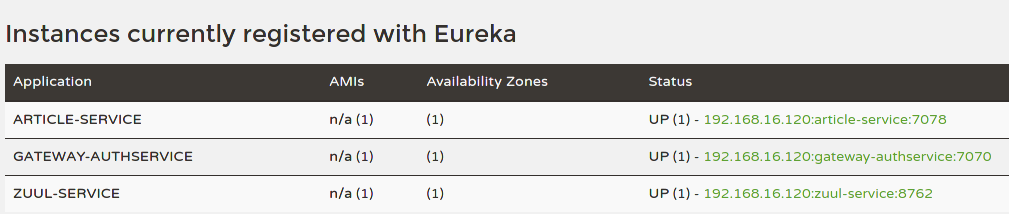
\includegraphics[width=\textwidth]{Eureka_Discovery.png}\label{fig:eureka_discovery}


\subsection{Eind beoordeling / reflectie}
Door het uitwerken van verschillende trends binnen zowel het individueel als het groepsproject oriënteer ik mijzelf
als "proficient" de bewijs last van het toepassen van deze technieken zijn zowel hierboven omschreven en terug te
vinden in de implementatie binnen de projecten.

\newpage
